\section{Super--resolution technology}
Super--resolution is a~group of techniques that upscale images and improve
their quality.
Such an algorithm can be treated as a function that takes an image and returns
it with a resolution \textit{n} times larger.
Algorithms taken into account in the process usually upscale images two or
three times.

It is important to distinguish between super--resolution and traditional
upscaling algorithms.
The later use interpolation to enlarge images; however, they hardly improve the
quality of the image.
The intent of super--resolution is not only to upscale images, but to improve
the quality and detailing.
Nowadays, such an effect is achieved using machine learning, precisely---deep
learning---a technology that utilizes multi--layered neural networks trained
with large datasets.
Deep learning networks that process image data usually utilize convolutional
layers.
Such layers contain a number of image filters that are tuned during training.
Like all the rest of machine learning algorithms, the deep learning based
super--resolution works in a statistical manner.
This means that the extra details created during the image enhancement process
state an imaginary approximation of image features.
It is important to keep the statistical nature of machine learning algorithms
in mind.

Two kinds of super--resolution algorithms can be outlined:
\textit{one--to--one} and \textit{many--to--one}.
The first one is the obvious approach, where one low--resolution image is
translated into high--resolution one.
The latter is more advanced technique, which utilizes multiple low--resolution
images of the same scene to produce one high resolution picture.
The usual approach is to have multiple low--resolution images that are slightly shifted.
Data from these multiple images is merged together to produce an image of greater quality.
This approach can lead to best results in super--resolution.
In some scenarios the data fusion can lead to recreation of high resolution details that are hardly visible in any single low--resolution image.
Moreover, it should be noticed that the super--resolution networks trained on
domain--specific data often cannot be used to enhance images with different
contents.
For example, if a network was trained on a dataset with human faces, it is
likely to perform poorly on satellite images.
Network architecture can also be domain--specific, for example, utilizing
different bands of a multispectral image.

Super--resolution imaging is a technique relevant in the fields of satellite imaging
remote sensing and geoscience.
The most common reason for image enhancement is for aesthetic reasons.
This application is viable in satellite imaging; however, super--resolution can
lead to other practical advantages.
Image enhancing techniques can be used as a preprocessing step in remote
sensing pipelines.
For this reason super--resolution can be especially useful when considered in
the context of satellite imagery.
A visual demonstration of modern super--resolution applied on satellite images can be seen in figures \ref{fig:super-res-fields-demo} and \ref{fig:super-res-dots-demo}.
In these examples a set of nine low--resolution images per each scene was super--resolved into a single high--resolution one.
A sample of those nine images is shown in the comparison.
\begin{figure}[p]
    \centering
    \begin{subfigure}[t]{0.31\textwidth}
        \centering
        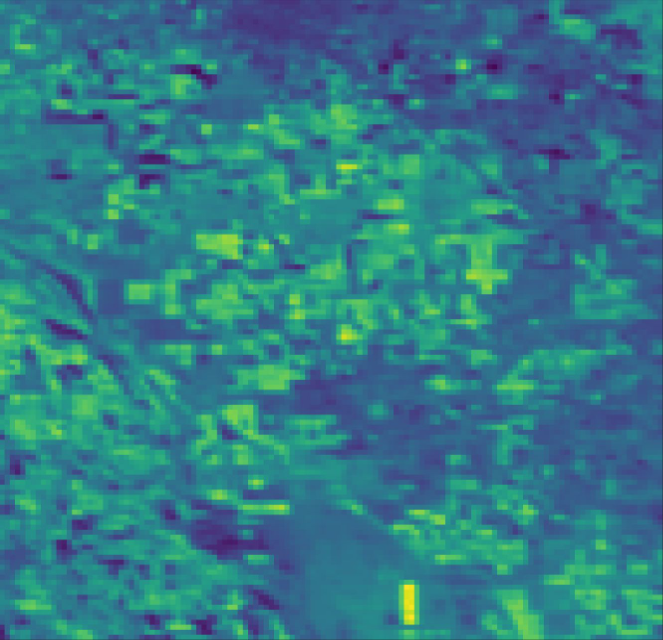
\includegraphics[width=\textwidth]{high_res_net_demo_fields_lr}
        \caption{One of nine low--resolution images}
    \end{subfigure}
    \hfill
    \begin{subfigure}[t]{0.31\textwidth}
        \centering
        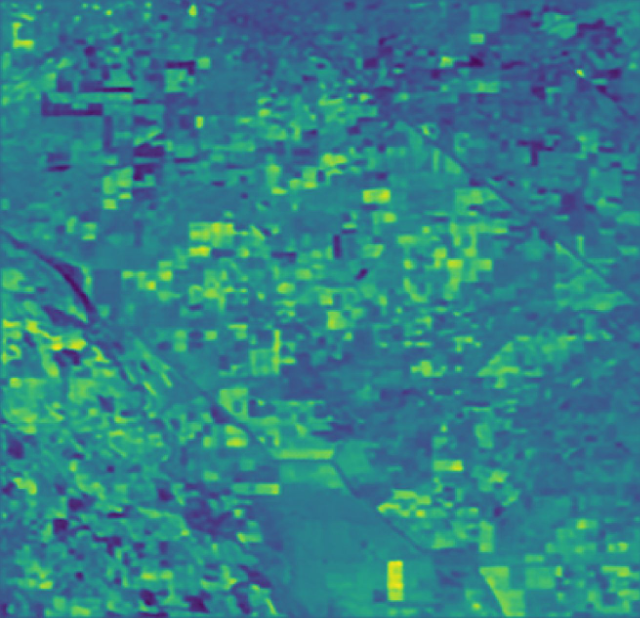
\includegraphics[width=\textwidth]{high_res_net_demo_fields_sr}
        \caption{Super--resolution reconstruction of the scene}
    \end{subfigure}
    \hfill
    \begin{subfigure}[t]{0.31\textwidth}
        \centering
        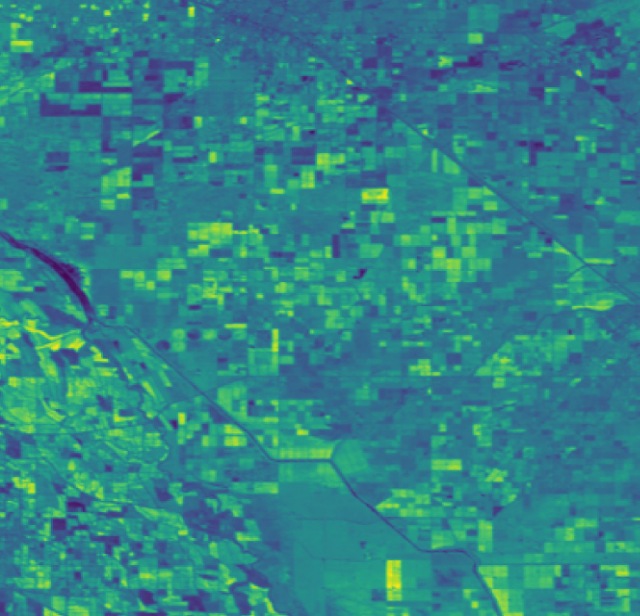
\includegraphics[width=\textwidth]{high_res_net_demo_fields_hr}
        \caption{Real--life high--resolution picture of the scene}
    \end{subfigure}
    \caption{A demonstration of super--resolution technique, where nine low--resolution satellite images of a farming area are turned into one  high--resolution image}
    \label{fig:super-res-fields-demo}
\end{figure}
\begin{figure}[p]
    \centering
    \begin{subfigure}[t]{0.31\textwidth}
        \centering
        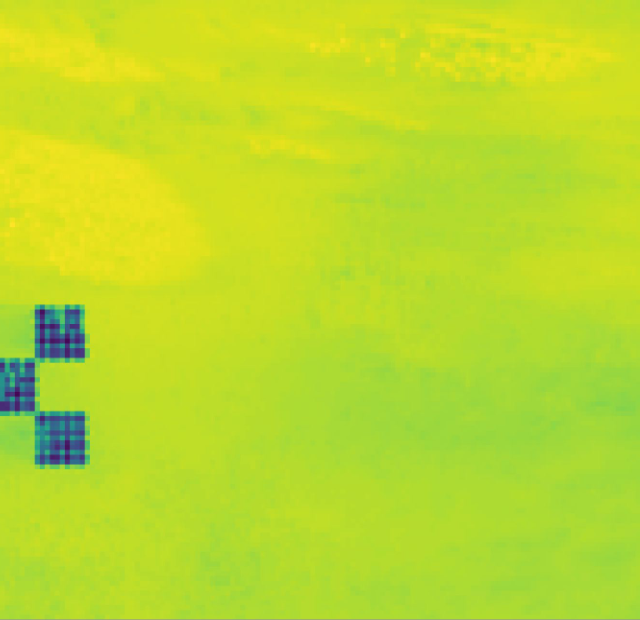
\includegraphics[width=\textwidth]{high_res_net_demo_dots_lr}
        \caption{One of nine low--resolution images}
    \end{subfigure}
    \hfill
    \begin{subfigure}[t]{0.31\textwidth}
        \centering
        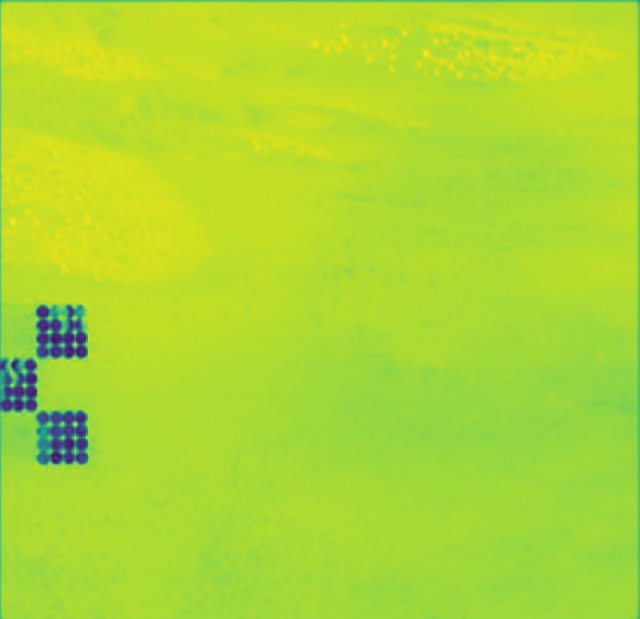
\includegraphics[width=\textwidth]{high_res_net_demo_dots_sr}
        \caption{Super--resolution reconstruction of the scene}
    \end{subfigure}
    \hfill
    \begin{subfigure}[t]{0.31\textwidth}
        \centering
        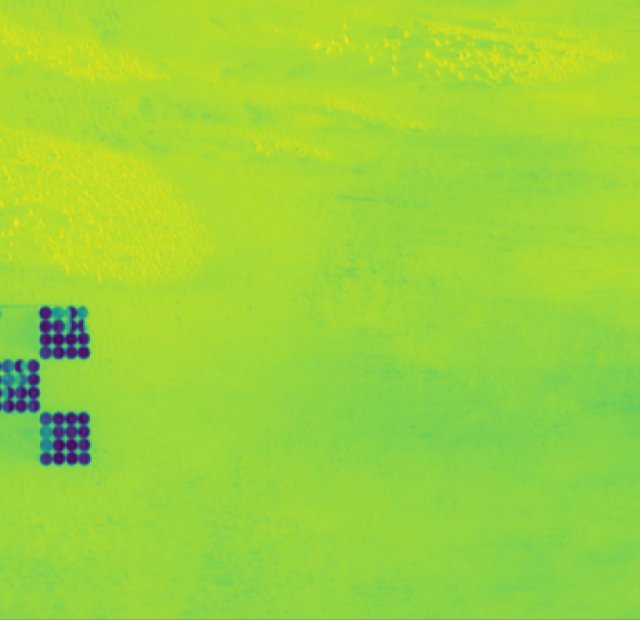
\includegraphics[width=\textwidth]{high_res_net_demo_dots_hr}
        \caption{Real--life high--resolution picture of the scene}
    \end{subfigure}
    \caption{A demonstration of super--resolution technique, where nine low--resolution satellite images of a barren landscape are turned into one  high--resolution image}
    \label{fig:super-res-dots-demo}
\end{figure}

\section{Purpose of data augmentation and available solutions}
Deep learning, utilized in the modern super--resolution techniques, requires a
lot of data to train successfully.
Increase in quality and size of dataset can lead to far better results when
training a neural network.
This is why data augmentation techniques are often used to improve performance
of deep networks.
Data augmentation incorporates various transformation to improve, multiply or
generate training data.
Data created in the augmentation process is often called \textit{synthetic}.
Common techniques to improve image data include zooming, resizing, shifting,
flipping, rotating, distorting, adding noise, modifying colors and exposure.
These operations may be application--specific.
To give an example, one should beware of distorting or flipping data containing with constrained geometry, like road signs.
The mentioned augmentation techniques can be considered classic and rather
trivial.
However, more advanced approach can be taken to generate data.
It is possible to create deep neural networks to create data augmentation
transformations.
This approach can be especially useful when a dataset is available that it is
too small to train the desired network.
A smaller network can be made and trained on an existing small dataset to multiply
the data.
Then the augmentation network can be used to generate more data for the
original model to learn.
With deep learning capabilities networks can learn to multiply, transform or
even generate data without direct input \cite{bulat-2018-supergan}.

\section{Aim of the work and motivation}
The objective of the work is to create a set of augmentation networks for
enhancing super--resolution training data.
Subsequent chapters will present considered super--resolution architectures
with greater details and propose neural network models for data augmentation.
The task of the augmentation algorithms is to create low--resolution images for
high--resolution ones, to make training pairs for super--resolution networks. 

The nature of super--resolution technology and satellite imagery imposes certain
ways in which data augmentation should be applied to the training data.
Super--resolution is trained using pairs of data---low resolution image with
high resolution image (or a set of low resolution images with high resolution
image in case of many--to--one network).
This requirement renders compiling training sets a challenge, especially in the
field of satellite imagery.
In such a scenario the most common technique is to use resizing algorithms on
single image datasets.
A set of training pairs can be created by downscaling high--resolution images.
In the case of many--to--one networks, a single high--resolution image can be
multiplied and shifted before shrinking to create more low--resolution images.
Such a technique may work well; however, it infuses the data with information
about resizing algorithms.
The way high--resolution and low--resolution images relate in such a set
depends on the interpolation algorithm (e.g., bicubic, bilinear,
nearest, lanczos).
The network trained on such datasets will likely learn to invert given
interpolation methods.
This does not match exactly real--life scenarios, most images are not created
using resizing algorithms.
Another approach utilizes pairs of real low--resolution and high--resolution
images of the same scene, taken by cameras of different quality.
The con of this method is challenging data acquisition process---satellite
images are rarely taken in pairs.
Such a dataset has to be deliberately made with super--resolution in mind,
which makes such data less common.
The main idea of the project is to use such a dataset of real--life data to
train an augmentation network.
Such a network would learn to create low--resolution images for
high--resolution, without imprinting resampling algorithms mechanisms into the
data.
The relation between low and high--resolution images in such an augmented
dataset would resemble the relation between same image taken by cameras of
different quality. 
The augmentation neural network can be then used on other satellite image
datasets to generate training data pairs for super--resolution.
Different data, models and generation techniques can be used to achieve desired
results.
Possible variations are discussed in the course of this work to improve
super--resolution datasets.